
\section{Information theory for closed loop controllers \label{Introduction:InfoTheoryClosedLoop}}

This section contains the essential background for the application of information
theory to closed loop controllers.
It will be used extensively for the computation of information measures in the 
following sections.

\subsection{Introduction: closed loop controllers}
In control theory there are two main approaches: feed-forward and feedback control. 
Feed-forward control is possible only when the law or transfer of the
 process I want to control is known. Natural systems are very hard to control
using the open loop approach because they are dynamic non-linear processes and
their parameters are subject to noise. Feedback control does not require
the full knowledge of the process and is based on the principle of action and reaction.
Adaptive controllers change their parameters according to the observed parameters of
the process to control: most biological organisms use the control loop approach.
The daily process of maintaining our body temperature is an example of such a system \citep{HumanBody}.
Until today cybernetics has provided a lot of adaptive controllers for the closed loop:
PID\nomenclature{PID}{Proportional Integration Derivative control} controllers
(see Figure \ref{Figure:maxcorr:PID}) and the Kalmann filter to mention the most important.

\begin{figure}[ht]
  \begin{center}
    \includegraphics[width=0.6 \textwidth]{maxcorr/InfoAgentTheory-2.eps}
    \caption[Classical proportional controller]{
	     A classical proportional controller described only by the gain $K$.
	      \label{Figure:maxcorr:PID}}
  \end{center}
\end{figure}
Artificial intelligence (AI) branched from cybernetics and used what was available
from the previous approaches, but it realised that designing artificial agents
for the real world using the previous
approaches was not possible: agents should use biological inspired behaviour to
operate in the real environment without any harm for other persons or entities.
Hebbian learning, neural networks, Q-learning, fuzzy logic and many others are
nowadays used in many artificial agent systems. However using these adaptive
controllers raises a big concern: how can I assess the performance of the agents?
The question is not as trivial as it seems: the agent adapts to the environment,
thus in general a more complex environment produce a more complex
behaviour \citep{NolfiInteraction}. 
But agents essentially perform input control to keep their desired state.
The only solution to that problem is to develop input based measures and not 
output based measures as I will demonstrate in Section \ref{Chapter5:Max Corr Input}.
Input contains the output of the agent through the environment,
therefore if the agent is learning, it means it is changing the inputs to achieve
a desired state (for example avoiding a painful signal).
This approach was introduced by \citet{Gibson1955:learning} who rejected
cognitivism and behaviourism for a more direct realism. 
He argued that organisms perform only input control, one of his most radical
 approach was the concept of ``affordances'' whereby the objects of our environment
 tell implicitly how they want to be operated.
Although there are some cases where organisms perform open loop forward control,
 the general principles described by Gibson are valid.
the general model is described in Figure \ref{Figure:maxcorr:Gibson}.

\begin{figure}[ht]
  \begin{center}
    \includegraphics[width=0.6 \textwidth]{maxcorr/InfoAgentTheory-4.eps}
    \caption[Gibson cybernetic approach]{
	     Model of perception as described by Gibson in 1955: the agent performs input control.
	     \label{Figure:maxcorr:Gibson}}
  \end{center}
\end{figure}

The theory of Shannon's information cannot be applied directly in closed loop
 systems because the information flow in an organism is asymmetric
(see Figure \ref{Figure:maxcorr:asymmetry}).
In the agent perspective the action is sensed via a representation of the
controlled process.

\begin{figure}[ht]
  \begin{center}
    \includegraphics[width=0.6 \textwidth]{maxcorr/InfoAgentTheory-3.eps}
    \caption[Information asymmetry in the organism]{
	     The problem of information asymmetry in the closed loop control case.
	      \label{Figure:maxcorr:asymmetry}}
  \end{center}
\end{figure}

In fact the traditional notion of Shannon entropy was extended by \citet{Touchette2004} to closed loop
systems by considering the sensory-motor loop as a communication channel which 
extends in time to propagate information from and to the environment.
For instance \citet{Touchette2004} revisited the idea of a controller as
 an actuation channel that transforms input states to desired output states.
He also gives necessary and sufficient conditions for a system to be perfectly
 controllable and perfectly observable in terms of information and entropy.
His model is a Bayesian network composed by a sensor channel $S$,
an actuator channel $A$, the initial state of the system $X$ and the final
state of the system $X'$. The model as described in Fig. \ref{fig:tishby1} both
represented in Shannon's terms by their probability distribution matrix $p(a|s)$,
where $s$ is the input random variable of the channel and $a$ the output random
variable of the channel.
The controller is modelled as a random variable $C$ that takes an initial state
 $X$ of the system to a final target state $X'$. A closed loop controller chooses
a regulation $a_i \in A$ based on the state of the system $x_i \in X$, whereas an open loop
 controller chooses a regulation $a_i \in A$ that is independent of the sate of the system $x_i \in X$.
Open loop control is thus different from a closed loop control in terms of
mutual information $I(X,C)$ as described in Eq. \ref{infotheory:eq:control}: 
\begin{eqnarray}
open \; loop &:& I(X;C)=0\\
closed \; loop&:& I(X;C)>0
\label{infotheory:eq:control}
\end{eqnarray}

\begin{figure}[!htbp]
\begin{center}
\includegraphics[width=0.8 \textwidth]{ashby/figure-2}
\caption[Bayes formulation in traditional control]{
Bayesian formulation of open and closed loop.
A) Full control model.
B) Reduced open loop model.
C) Reduced closed loop model.
D) Single actuation channel model.
The only way to distinguish open loop from closed loop is by means of Eq. \ref{infotheory:eq:control}.
\label{fig:tishby1}
}
\end{center}

\end{figure}

The controller can be extended for the predictive case introduced in section \ref{Introduction:NeuralSystem},
by adding an additional variable $Y$ which is the predictor of $X$ as in Fig. \ref{fig:tishby2}:
$Y$ conveys information about $X$ and is used by the controller to infer the 
temporal relation between the predictor $Y$ and the reflex $X$.
This Bayesian model is investigated more in depth in section \ref{Conclusion:PredictiveBayes}.
\begin{figure}[!htbp]
\begin{center}
 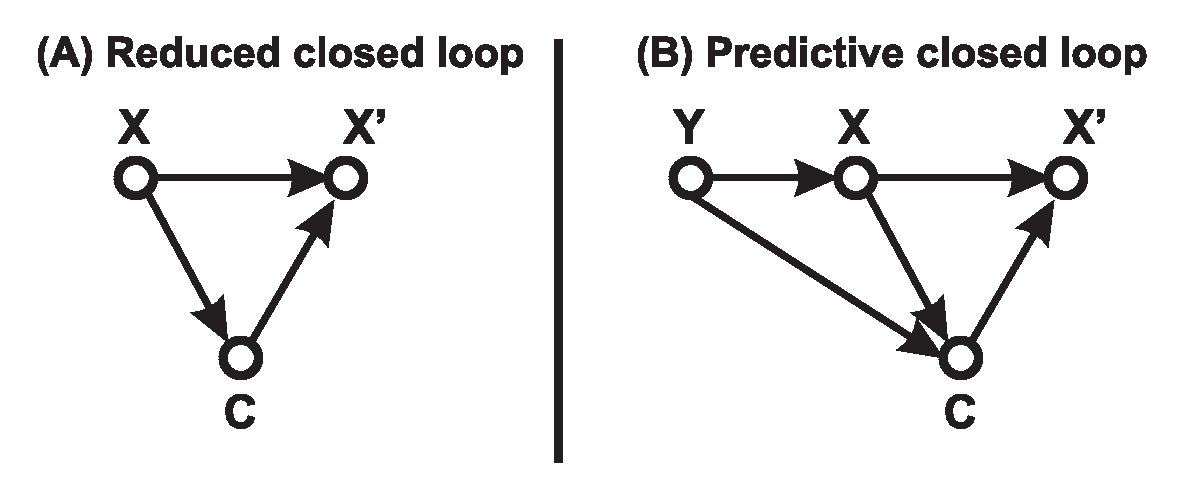
\includegraphics[width=0.8 \textwidth]{ashby/figure-4}
\caption[Bayes formulation in predictive control]{
Extended Bayesian formulation.
\textbf{A)} open loop case with sensor collapsed into controller $S=C$.
\textbf{B)} closed predictive loop with $Y$ predictive signal on $X$.
\label{fig:tishby2}}
\end{center}
\end{figure}

Other important tools were provided by \citet{Tishby1999:InfoBottle} with the 
the information bottleneck method which considers the ability of learning 
in predictive controllers related to the compression achieved when two or more
signals are mutually dependent.

The first practical application of information measures to closed loop controllers
was introduced by \citet{organizationInfo} who used the Tishby's framework
to implement an information based controller as described in Fig. \ref{fig:conclusion:polani}.
The approach used is similar to the one described in Fig. \ref{Figure:maxcorr:asymmetry} 
but with an optimization value provided by the information flow: the controller's
transfer function is a model of the environment and the goal of the controller
consists in maximizing the information flow from the motor output to the sensory input.
With this very general approach the controller is able to achieve meaningful states
without even defining a task objective.
The disadvantage of the approach is that the controller needs to have a good model
of the environment and needs to be able to do simulations and choose the best
path to maximize the information flow.


\begin{figure}[htbp]
\begin{center}
\includegraphics[scale=0.3]{figures/conclusion/polani2008.eps}
\end{center}
\vspace*{4pt}
\caption[Empowerment from Polani]{
The empowerment is defined as the maximum information flow
from the action $A_{t}$ to the sensors $S_{t+1}$ via the environment $R_{t}$.
The source of uncorrelated randomness $Z_{t}$ is useful to assess the controllability
when the organism is removed from the control law.
\label{fig:conclusion:polani}}
\end{figure}

A more general approach was introduced by \citet{LungarellaInformation} who
used several information based metrics to follow the learning curve of the robot
in a visual foveation task: the robot reduces the entropy around the centre of focus.
\citet{LungarellaInformation} describe a closed loop system as a system that
decreases the entropy, increases the information structure (statistical regularity),
decreases the complexity.

A similar approach was used by \citet{Ay2008:PredInformation} to modify the proportional
coefficient in the controller's function to allow an optimal exploration strategy
of an environment with obstacles: the mutual information between past and future
is used to tune the gain $c$ so that the maximum of the predictive information defines the best exploratory
behaviour.

The next section contains an overview of Ashby's framework which will be used in this thesis.

\subsection{Regulation and entropy \label{Appendix:Ashby}}
The main contribution earlier than Tishby to the cybernetic theory of controllers
was produced by Ashby in 1956 and it will be used heavily in this thesis.
\citet{Ashby1956:IntroCybernetics} defined clearly that the
 essential feature of a good regulator is to block the flow of variety from
disturbances to essential variables. Ashby uses variety precisely as the number
 of different states a variable can be and so it relates to Shannon's entropy:
if a variable has a variety of 4 states, then it can be described with 2 bits in terms of Shannon's entropy.
Thus variety and entropy can be used alternatively.
I use the same notation by Ashby so that it will be more clear how those concepts
can be applied successfully to predictive learning:
\begin{itemize}
 \item D is the domain of disturbances from the environment like a threat for an organism.
 \item E is the domain of the essential variable, can be partitioned in
$E= \eta \cup \overline{\eta}$, where $\eta$ is a partition of desired states
 or goals of the organism and its complementary partition $\overline{\eta}$
 represents the non-desired states.
 \item R is the domain of available regulations that the organism can perform
 \item T is the domain of the possible states of the environment.
 \item F is the combination of R and T.
\end{itemize}
The disturbance D tends to drive E outside the set of desired states $\eta$.
For open loop control systems the relationship between the mentioned variables 
is shown in Fig.\ref{fig:infotheory:ashby-model}(A).
Fig.\ref{fig:infotheory:ashby-model}(B) describes how the disturbance is absorbed by the regulator
 and the environment to keep a desired state.
\begin{figure}[!htbp]
\begin{center}
 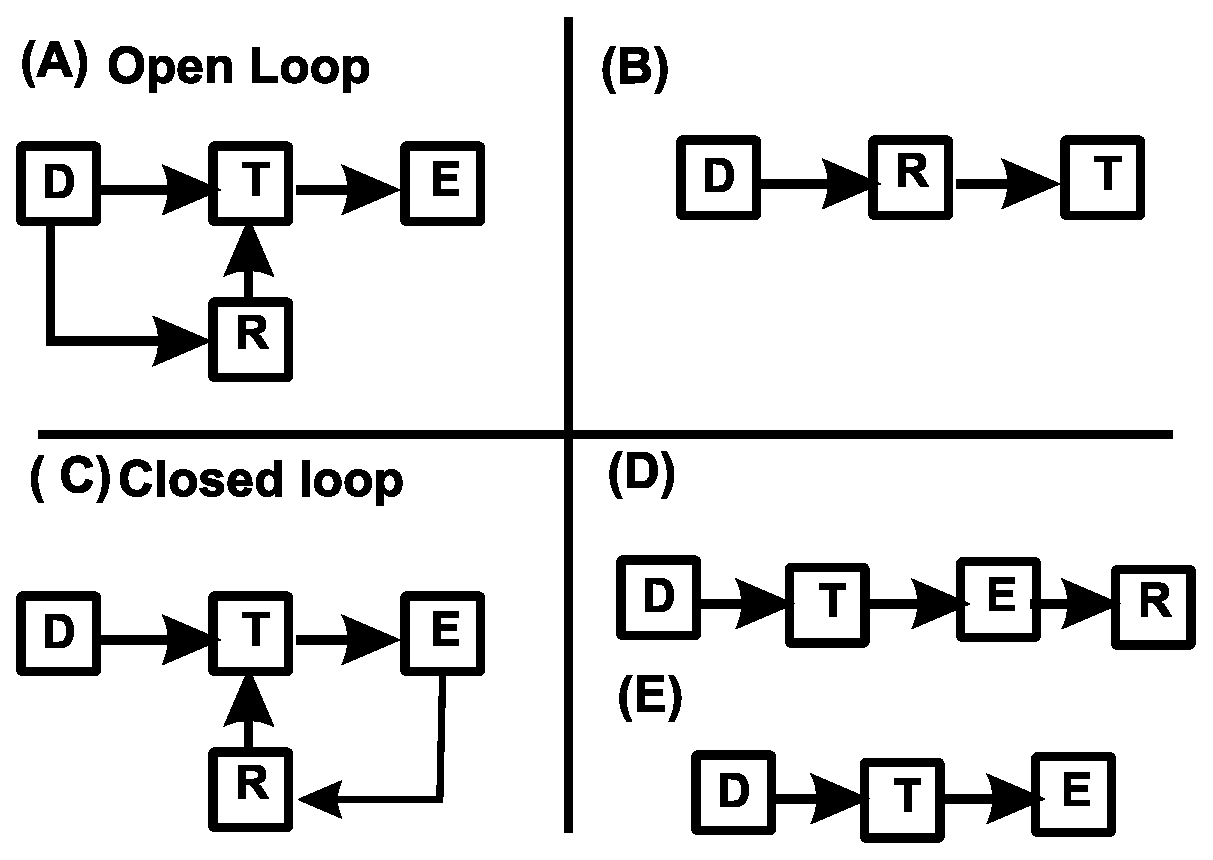
\includegraphics[width=0.6 \textwidth]{ashby/figure-1}
\caption[Ashby requisite variety]{Ashby's law of requisite variety \citep{Ashby1956:IntroCybernetics} applied 
to the open loop case (A),(B) and the closed loop case (C),(D).
\label{fig:infotheory:ashby-model}
}
\end{center}
\end{figure}

Figure \ref{fig:infotheory:ashby-model}(C)(D) describes how the disturbance is absorbed by the regulator
 and the environment to keep a desired state in a closed loop configuration.

The problem of regulation is defined as follows: 
given E,$\eta$, T, and D, to form the mechanism R so that R and T, coupled, 
act to keep E within $\eta$.

\subsection{Direct regulation}
Ashby described direct regulation as a control strategy similar to what engineers
call open loop control.
The update rule for the direct regulation of Figure \ref{fig:infotheory:ashby-model}(A) follows:
\begin{itemize}
 \item D generates a disturbance $d(t)$
 \item $d(t)$ is the input to R which outputs $r(t)$
 \item the 2 values $d(t),r(t)$ are inputs to $T$ that produces $e(t)$
 \item the value $e(t)$ is a state in $E$ which can be a desired or non desired state
\end{itemize}
In the animal world, regulations in simple animals are direct: the organism reacts to the disturbance $D$ before it affects $E$.
A good example is in the life cycle of frogs: tadpoles reacts to a touch stimulus (for example
when a person poke them with a finger) with a swimming reaction opposite to the
direction of the stimulus.
After some time the tadpole will stop swimming: there is no way for the animal
to check if the disturbance was still there.

Most often in the animal world, the R's action cannot be completed before the output of T
is known: the regulator does not know the disturbance directly but only through
the environment or after the organism has experienced the disturbance.


\subsection{Closed loop regulation}
The closed loop regulation is defined when R receives its input from E and not from T
as in Figure \ref{fig:infotheory:ashby-model}(C).
The regulator does not receive directly the disturbance but only after it passed
the environment or the organism.

\begin{figure}
\begin{center}
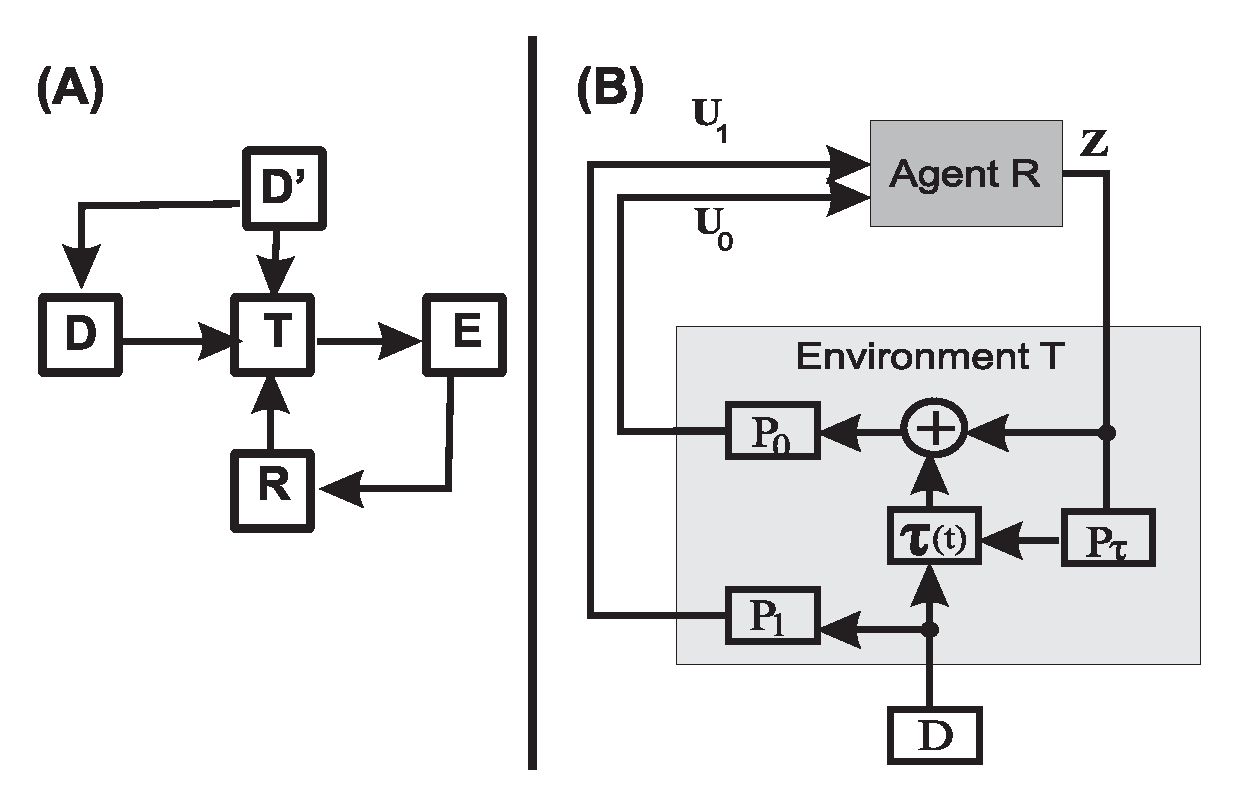
\includegraphics[width=0.8\textwidth]{ashby/figure-3}
\caption[Ashby law in predictive controllers]{
Ashby law of requisite variety applied to the ICO learning controller
\label{fig:infotheory:ashby2}}
\end{center}
\end{figure}

The special case of a predictive controller was not considered by Ashby and therefore
it will be necessary to formulate the necessary conditions for learning.
A possible extension of the Ashby's variety for the ICO controller is in Fig. \ref{fig:infotheory:ashby2}
on the right side there is the ICO controller of the robot and on the left side
there is the corresponding machine state model.
In Fig. \ref{fig:infotheory:ashby2}(A) the disturbance $D'$ is a predictor of $D$ and goes
through the environment $T$ affecting the essential variables $E$ of the controller.
In Fig. \ref{fig:infotheory:ashby2}(B) the diagram of the ICO controller 
This novel approach to predictive controllers is going to be investigated in Section \ref{Chapter8:Predictive Performance}.
In the rest of this section, the original formulation of Requisite Variety is 
introduced.

\subsection{The law of requisite variety}
Please note that with the same notation D,E,R,T,F in the diagrams, I refer to
 the determinate or indeterminate (Markovian) closed transformation whose
allowed states are present in the corresponding domains.
\textbf{Definition of regulation:} an organism is a perfect regulator if
is able to keep the essential variables in a desired set $\eta$ in spite
of the disturbances.
\textbf{Regulation blocks the flow of entropy: } if F is a regulator, the insertion
of F between D and E decreases the variety that is transmitted from D to E.
How do we measure the performance of R as a regulator?
\textbf{The function of the regulator R is to reduce the entropy that is transmitted
 from D to E allowing the organism to be in the $\eta$ partition of desired states.}
Thus if F is missing the organism will likely experience the entire set $E$, with
a variety $H(E)$ but when F is introduced, the variety will be reduced to $H(\eta)<H(E)$.
Thus a perfect regulator will prevent the organism from knowing in what state the
disturbance was: the information channel that goes from the disturbance to the
essential variables is blocked totally by the regulator.

The law of requisite variety in terms of Shannon's entropy:
\begin{quotation}
The law of requisite variety says that R's capacity as a regulator cannot
exceed R's capacity as a channel of communication.
It can be formulated in Shannon's terms assuming that: $D$ is the noise that is
 being transmitted to $E$ the essential variables of the organism by means of $T$
the environment, $R$ the regulator is a correction channel whose input is $D$ and
whose output is $T$ whose role is to reduce the variety in the $E$ channel.
In an ideal case $H(E)=0$ such that $H(D)=H(R)$, the regulator must have
the same variety as the disturbance. 
\end{quotation}

\subsection{First law of requisite variety}
Let $D,R$ and $E$ be three random variables.
\textbf{Hypothesis:} when $R$ is given, the entropy of $E$ cannot be less then that of D: $H(E|R)\geq H(D|R)$.
Then the role of the organism is to achieve maximum control over its internal variable E,
thus reducing the uncertainty.
The minimum possible regulation that can be achieved is $H(D)+H(R|D)-H(R)$:
\begin{equation}
H(E)\geq H(D)+H(R|D)-H(R) \label{variety:eq:minh}
\end{equation}
\paragraph{Corollary 1:}
if R is a determinate function of D: $H(R|D)=0$, the minimum entropy of E is $H(D)-H(R)$.
The first law of requisite variety says that E's entropy can only be reduced by
 an equal increase in R's variety.
Proof:\\
For the chain rule of entropy:
\begin{equation}
H(R,D)=H(D)+H(R|D)=H(R)+H(R|D)
\end{equation}
substitute $H(E|R)$ for $H(D|R)$ in previous equation gives:
\begin{eqnarray}
H(D)+H(R|D) \leq H(R)+H(R|E)\\
H(D)+H(R|D) \leq H(R,E)\\
H(R,E) \leq H(R)+H(E)\\
H(D) +H(R|D)\leq H(R)+H(E)\\
H(E) \geq H(D) +H(R|D)-H(R)
\end{eqnarray}
The corollary was demonstrated in \citet{Ashby1956:IntroCybernetics}.

\subsection{Second law of requisite variety}
Let D,R and E be three random variables.
Hypothesis: when $R$ is given, the entropy of E cannot be less then that of
 D minus a constant K: $H(E|R)\geq H(D|R)-K$.
Then the minimum entropy of E is $H(D)+H(R|D)-H(R)+K$:
\begin{equation}
H(E)\geq H(D)+H(R|D)-H(R)+K
\end{equation}
The constant K is here used to model the ``handicap'' of the organism.


